\documentclass[12pt,a4paper]{article}

% -------------------------------------------------
% Packages
% -------------------------------------------------
\usepackage[a4paper,margin=1in]{geometry}
\usepackage{amsmath,amssymb,amsthm}
\usepackage{tikz}
\usepackage{mathtools}
\usepackage{physics}

% -------------------------------------------------
% TikZ libraries
% -------------------------------------------------
\usetikzlibrary{
    arrows.meta,
    positioning,
    calc
}

% -------------------------------------------------
% Useful commands
% -------------------------------------------------
\newcommand{\Z}{\mathbb{Z}}
\newcommand{\R}{\mathbb{R}}
\newcommand{\ee}{\mathrm{e}}

% -------------------------------------------------
% Document
% -------------------------------------------------
\begin{document}

\begin{center}
    {\Large \textbf{HW1: QFT I}}\\[4pt]
    {\large Erfan Najafian}
\end{center}

\vspace{0.5cm}

% =================================================
% 1. Lattice and path representation
% =================================================

\section*{1. Lattice and Paths}

For a $d$-dimensional lattice, we define

\begin{equation}
    x^\mu = n^\mu \Delta,
    \qquad
    n^\mu \in \mathbb{Z}^d .
\end{equation}

For example, in two dimensions there are two independent lattice
directions,

\begin{equation}
    \hat e_1,\qquad \hat e_2,
\end{equation}

and in three dimensions,

\begin{equation}
    \hat e_1,\qquad
    \hat e_2,\qquad
    \hat e_3.
\end{equation}

In general, for four dimensions,

\begin{equation}
    \hat e_i,
    \qquad i=1,2,3,4.
\end{equation}

% -------------------------------------------------
% 2D lattice figure
% -------------------------------------------------

\begin{figure}[h!]
\centering

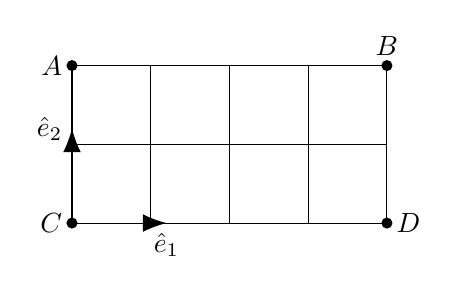
\begin{tikzpicture}[scale=1.0]

% Grid
\draw[thin] (0,0) grid (4,2);

% Outer points
\fill (0,0) circle (2pt);
\fill (0,2) circle (2pt);
\fill (4,2) circle (2pt);
\fill (4,0) circle (2pt);

% Labels
\node[left]  at (0,2) {$A$};
\node[above] at (4,2) {$B$};
\node[left]  at (0,0) {$C$};
\node[right] at (4,0) {$D$};

% Coordinate axes
\draw[-{Latex[length=3mm]}] (0,0) -- (1.2,0)
    node[below] {$\hat e_1$};

\draw[-{Latex[length=3mm]}] (0,0) -- (0,1.2)
    node[left] {$\hat e_2$};

\end{tikzpicture}

\caption{A two-dimensional lattice.}
\end{figure}

The number of independent directions in $d$ dimensions is $d$.
For example,

\begin{equation}
    d=2
    \quad\Longrightarrow\quad
    \mu=1,2,
\end{equation}

while

\begin{equation}
    d=3
    \quad\Longrightarrow\quad
    \mu=1,2,3.
\end{equation}

% -------------------------------------------------
% 3D lattice
% -------------------------------------------------

\begin{figure}[h!]
\centering

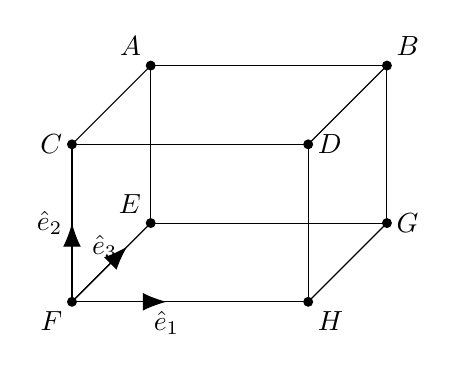
\begin{tikzpicture}[scale=1.0]

% Front square
\coordinate (F) at (0,0);
\coordinate (H) at (3,0);
\coordinate (D) at (3,2);
\coordinate (C) at (0,2);

% Back square
\coordinate (E) at (1,1);
\coordinate (G) at (4,1);
\coordinate (B) at (4,3);
\coordinate (A) at (1,3);

% Cube
\draw (F)--(H)--(D)--(C)--cycle;
\draw (E)--(G)--(B)--(A)--cycle;

\draw (F)--(E);
\draw (H)--(G);
\draw (D)--(B);
\draw (C)--(A);

% Vertices
\foreach \p in {A,B,C,D,E,F,G,H}
    \fill (\p) circle (1.8pt);

% Labels
\node[above left]  at (A) {$A$};
\node[above right] at (B) {$B$};
\node[left]        at (C) {$C$};
\node[right]       at (D) {$D$};
\node[above left]  at (E) {$E$};
\node[below left]  at (F) {$F$};
\node[right]       at (G) {$G$};
\node[below right] at (H) {$H$};

% Basis vectors
\draw[-{Latex[length=3mm]}]
    (F) -- ++(1.2,0)
    node[below] {$\hat e_1$};

\draw[-{Latex[length=3mm]}]
    (F) -- ++(0,1.0)
    node[left] {$\hat e_2$};

\draw[-{Latex[length=3mm]}]
    (F) -- ++(0.7,0.7)
    node[left] {$\hat e_3$};

\end{tikzpicture}

\caption{A three-dimensional lattice and its basis vectors.}
\end{figure}

Thus, in general,

\begin{equation}
    x^\mu=n^\mu\Delta,
    \qquad
    n^\mu\in\mathbb{Z}^d.
\end{equation}

The Green function can be represented as a sum over all paths
connecting the origin to $x$:

\begin{equation}
    \boxed{
    G(m_0,x)
    =
    \sum_{0\to x}
    \ee^{-m_0\,\ell(\text{path})}
    }
\end{equation}

where $\ell(\text{path})$ denotes the length of the path.

% =================================================
% 2. Simple example
% =================================================

\section*{2. Example}

Consider a path from $A$ to $C$. There are two shortest paths:

\begin{equation}
    A\longrightarrow B\longrightarrow C,
\end{equation}

and

\begin{equation}
    A\longrightarrow D\longrightarrow C.
\end{equation}

The corresponding diagram is

\begin{figure}[h!]
\centering

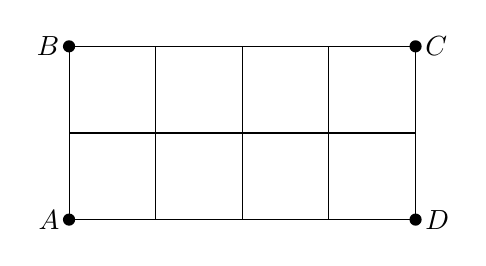
\begin{tikzpicture}[scale=1.1]

% Square
\coordinate (A) at (0,0);
\coordinate (B) at (0,2);
\coordinate (C) at (4,2);
\coordinate (D) at (4,0);

\draw[thin] (A)--(B)--(C)--(D)--cycle;

% Internal lattice
\draw[thin] (1,0)--(1,2);
\draw[thin] (2,0)--(2,2);
\draw[thin] (3,0)--(3,2);
\draw[thin] (0,1)--(4,1);

% Vertices
\foreach \p in {A,B,C,D}
    \fill (\p) circle (2pt);

\node[left] at (A) {$A$};
\node[left] at (B) {$B$};
\node[right] at (C) {$C$};
\node[right] at (D) {$D$};

\end{tikzpicture}

\caption{Two shortest paths from $A$ to $C$.}
\end{figure}

Therefore,

\begin{equation}
    A\to C
    \equiv
    \left\{
    \begin{array}{l}
    A\to B\to C,\\[2mm]
    A\to D\to C.
    \end{array}
    \right.
\end{equation}

Each shortest path has two lattice steps, so that

\begin{equation}
    \ell(\text{path})=2\Delta .
\end{equation}

Hence the contribution from these two paths is

\begin{align}
    G
    &=
    \sum_{A\to C}
    \ee^{-m_0\ell(\text{path})}
    \\
    &=
    \ee^{-m_0(2\Delta)}
    +
    \ee^{-m_0(2\Delta)}
    \\
    &=
    2\ee^{-2m_0\Delta}.
\end{align}

More generally, let $N_j(n)$ denote the number of paths of length
$j$ connecting the origin to the lattice point $n$. Then

\begin{equation}
    \boxed{
    G(m_0,n)
    =
    \sum_{j=0}^{\infty}
    N_j(n)\,
    \ee^{-m_0j\Delta}
    }
\end{equation}

% =================================================
% 3. Continuum limit
% =================================================

\section*{3. Continuum Limit}

Since

\begin{equation}
    n=\frac{x}{\Delta},
\end{equation}

we can write

\begin{equation}
    G(x,m_0)
    =
    \sum_{j=0}^{\infty}
    N_j\left(\frac{x}{\Delta}\right)
    \ee^{-m_0j\Delta}.
\end{equation}

In the continuum limit,

\begin{equation}
    \Delta\rightarrow0,
\end{equation}

we therefore have

\begin{equation}
    G(x,m_0)
    =
    \lim_{\Delta\to0}
    \sum_{j=0}^{\infty}
    N_j\left(\frac{x}{\Delta}\right)
    \ee^{-m_0j\Delta}.
\end{equation}

The number of paths grows as the lattice becomes finer. Therefore,
the mass parameter has to be treated carefully in the continuum
limit. In particular, we allow

\begin{equation}
    m_0=m_0(\Delta).
\end{equation}

The small-$\Delta$ expansion is

\begin{equation}
    \boxed{
    m_0(\Delta)
    =
    m_0(0)
    +
    \left.
    \frac{dm_0}{d\Delta}
    \right|_{\Delta=0}\Delta
    +\mathcal{O}(\Delta^2)
    }.
\end{equation}

% =================================================
% 4. Expansion of the exponential
% =================================================

\section*{4. Expansion}

We have

\begin{align}
    \ee^{-m_0(\Delta)j\Delta}
    &=
    \ee^{-m_0(0)j\Delta}
    \exp\left[
        -j\Delta
        \left(
        \left.
        \frac{dm_0}{d\Delta}
        \right|_{\Delta=0}\Delta
        +\cdots
        \right)
    \right].
\end{align}

Keeping the leading terms,

\begin{equation}
    \ee^{-m_0(\Delta)j\Delta}
    \simeq
    \ee^{-m_0(0)j\Delta}
    \left[
        1
        -
        j
        \left.
        \frac{dm_0}{d\Delta}
        \right|_{\Delta=0}
        \Delta
        +\cdots
    \right].
\end{equation}

Consequently,

\begin{align}
G(x,m_0)
\simeq
&
\sum_{j=0}^{\infty}
\ee^{-m_0(0)j\Delta}
\left[
N_j\left(\frac{x}{\Delta}\right)
+
jN_j\left(\frac{x}{\Delta}\right)
\left.
\frac{dm_0}{d\Delta}
\right|_{\Delta=0}
\Delta
\right]
\\
&\qquad
+\mathcal{O}(\Delta^2).
\end{align}

The change in the number of paths can be written schematically as

\begin{equation}
    \Delta N_j
    \simeq
    x\frac{dN_j}{dn}.
\end{equation}

Thus the behavior of $N_j(n)$ as $n\to\infty$ becomes important in
the continuum limit.

% =================================================
% 5. Fourier representation
% =================================================

\section*{5. Fourier Representation}

For a translationally invariant lattice, one may introduce a Fourier
representation of the path-counting function. Schematically,

\begin{equation}
    \ee^{ik_\mu x^\mu}
    =
    f(x),
\end{equation}

and the behavior of $N_j(n)$ for large $n$ determines the continuum
behavior of the Green function.

The important point is that as

\begin{equation}
    \Delta\rightarrow0,
\end{equation}

the lattice point

\begin{equation}
    n=\frac{x}{\Delta}
\end{equation}

goes to infinity for fixed nonzero $x$. Therefore, the asymptotic
growth of $N_j(n)$ has to be compensated by the exponential factor
in the propagator.

% =================================================
% 6. Number of paths
% =================================================

\section*{6. Growth of the Number of Paths}

Consider the Green function

\begin{equation}
    \boxed{
    G(m_0,x)
    =
    \sum_{j=0}^{\infty}
    N_j\left(\frac{x}{\Delta}\right)
    \ee^{-m_0j\Delta}
    }.
\end{equation}

A path of length $j$ contains $j$ elementary steps. In two
dimensions there are four possible nearest-neighbor directions,

\begin{equation}
    \pm\hat e_1,
    \qquad
    \pm\hat e_2,
\end{equation}

so that at each step there are at most

\begin{equation}
    2d=4
\end{equation}

possible choices.

In the same way, in four dimensions the number of nearest-neighbor
directions is

\begin{equation}
    2d=8.
\end{equation}

Thus the number of possible paths grows exponentially. For the
four-dimensional case,

\begin{equation}
    N_{2L}(x)\gtrsim 8^L,
\end{equation}

and in particular,

\begin{equation}
    N_{2L}(0)\gtrsim 8^L.
\end{equation}

This exponential growth is the source of the divergence of the
path sum unless the exponential suppression from the factor
$\ee^{-m_0j\Delta}$ is sufficiently strong.

% =================================================
% 7. Divergence condition
% =================================================

\section*{7. Condition for Convergence}

Starting from

\begin{equation}
    G(m_0,x)
    =
    \sum_{j=0}^{\infty}
    N_j(n)\,
    \ee^{-m_0j\Delta},
\end{equation}

and using the estimate

\begin{equation}
    N_{2L}(x)\gtrsim 8^L,
\end{equation}

we obtain

\begin{align}
    G(m_0,x)
    &\gtrsim
    \sum_{L=0}^{\infty}
    8^L
    \ee^{-m_0\Delta(2L)}
    \\
    &=
    \sum_{L=0}^{\infty}
    \left(
        8\ee^{-2m_0\Delta}
    \right)^L.
\end{align}

Therefore, convergence requires

\begin{equation}
    8\ee^{-2m_0\Delta}<1.
\end{equation}

Equivalently,

\begin{align}
    \ee^{-2m_0\Delta}
    &<
    \frac{1}{8},
\end{align}

which gives

\begin{align}
    -2m_0\Delta
    &<
    -\ln 8,
\end{align}

and hence

\begin{equation}
    \boxed{
    m_0
    >
    \frac{\ln 8}{2\Delta}
    }.
\end{equation}

Thus the bare mass parameter must grow appropriately as
$\Delta\rightarrow0$ in order to suppress the exponential growth
of the number of lattice paths.

% =================================================
% 8. Path illustration
% =================================================

\section*{8. Path Representation}

The sum over paths can be illustrated schematically as follows.

\begin{figure}[h!]
\centering

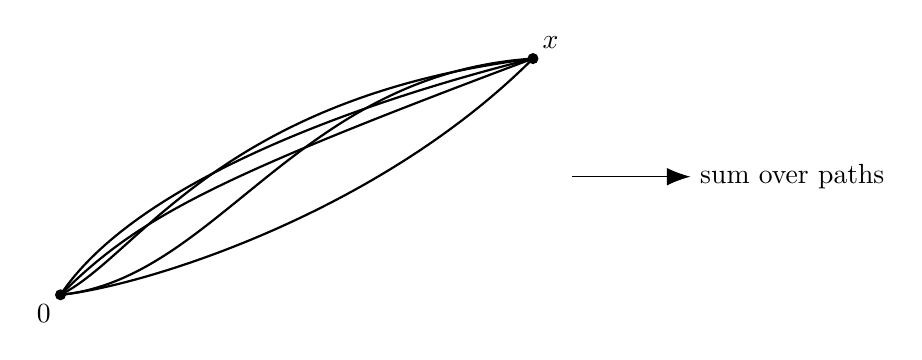
\begin{tikzpicture}[scale=1.0]

% Start and end points
\coordinate (O) at (0,0);
\coordinate (X) at (6,3);

% Several paths
\draw[thick]
    (O)
    .. controls (1,0.5) and (2,2.5) ..
    (X);

\draw[thick]
    (O)
    .. controls (1,1.0) and (2,1.5) ..
    (X);

\draw[thick]
    (O)
    .. controls (2,0.2) and (3,2.8) ..
    (X);

\draw[thick]
    (O)
    .. controls (1,0.1) and (4,1.0) ..
    (X);

\draw[thick]
    (O)
    .. controls (1,1.5) and (4,2.5) ..
    (X);

% Points
\fill (O) circle (2pt);
\fill (X) circle (2pt);

\node[below left] at (O) {$0$};
\node[above right] at (X) {$x$};

% Arrow
\draw[-{Latex[length=3mm]}]
    (6.5,1.5) -- (8,1.5)
    node[right] {sum over paths};

\end{tikzpicture}

\caption{Schematic representation of paths from $0$ to $x$.}
\end{figure}

Hence the Green function is the weighted sum

\begin{equation}
    G(m_0,x)
    =
    \sum_{\text{paths }0\to x}
    \ee^{-m_0\ell(\text{path})}.
\end{equation}

Each path is weighted by its length, and the factor
$\ee^{-m_0\ell}$ suppresses long paths.

% =================================================
% AI Assistance
% =================================================

\subsection*{AI-Assisted Preparation}

This document was prepared with the assistance of
\textbf{ChatGPT (GPT-5.6 Luna)}, an artificial intelligence model
developed by \textbf{OpenAI}. The assistance included
transcription and formatting of the handwritten material,
LaTeX typesetting, organization of the equations, and
reconstruction of the diagrams using TikZ.

The mathematical content is based on the original submitted
material.
\end{document}